\addcontentsline{toc}{section}{Introduction}

\section*{Introduction}
Dans ce chapitre, nous examinerons en détail les technologies clés qui sont utilisées dans notre solution pour fournir des fonctionnalités avancées et répondre aux besoins spécifiques de notre projet. Les trois principales technologies que nous aborderons sont Delta Lake, Trino et les Microfrontends.

\section{Delta Lake}

Delta Lake est une technologie de gestion des données qui permet de stocker, gérer et analyser des volumes massifs de données de manière efficace et fiable. Il repose sur une architecture basée sur des fichiers parquet et offre des fonctionnalités avancées telles que la gestion des transactions ACID (Atomicité, Cohérence, Isolation, Durabilité) et la compatibilité avec des outils d'analyse populaires. Delta Lake garantit également l'intégrité des données, la cohérence des requêtes et la prise en charge de la réplication et de la récupération en cas de défaillance.

Le concept de "lakehouse" est rendu possible grâce à Delta Lake. Il s'agit d'une architecture de données qui combine les avantages des entrepôts de données et des lacs de données, en offrant une approche unique et cohérente pour la gestion des données. Les données sont stockées au format Parquet dans le lac de données, permettant ainsi un traitement continu et par lots.
\begin{itemize}
    \item \textbf{Permet une architecture Lakehouse:} Delta Lake permet une architecture de données continue et simplifiée qui permet aux organisations de gérer et de traiter d'énormes volumes de données en continu et par lots sans les tracas de gestion et d'exploitation liés à la gestion séparée du streaming, des data warehouses et des lacs de données.
    \item \textbf{Permet une gestion intelligente des données pour les lacs de données:} Delta Lake offre une gestion efficace et évolutive des métadonnées, qui fournit des informations sur les volumes de données massifs dans les lacs de données. Grâce à ces informations, les tâches de gouvernance et de gestion des données se déroulent plus efficacement.
    \item \textbf{Application du schéma pour une meilleure qualité des données:} Étant donné que les lacs de données n'ont pas de schéma défini, il devient facile pour les données mauvaises/incompatibles d'entrer dans les systèmes de données. La qualité des données est améliorée grâce à la validation automatique du schéma, qui valide la compatibilité DataFrame et table avant les écritures.
    \item \textbf{Permet la transaction ACID:} La plupart des architectures de données organisationnelles impliquent de nombreux mouvements ETL et ELT entrant et sortant du stockage de données, ce qui l'ouvre à plus de complexité et d'échecs aux points d'entrée des nœuds. Delta Lake garantit la durabilité et la persistance des données pendant l'ETL et d'autres opérations de données. Delta Lake capture toutes les modifications apportées aux données pendant les opérations de données dans un journal des transactions, garantissant ainsi l'intégrité et la fiabilité des données pendant les opérations de données.
\end{itemize}

\section{Avantages de Delta Lake}
\begin{flushleft}
	Avec Delta Lake, les données sont stockées dans un format optimisé, tel que Parquet, dans un lac de données. Ce format facilite le traitement efficace des requêtes, quel que soit le mode d'accès aux données, qu'il s'agisse d'un traitement streaming ou par batch.
\end{flushleft}

\begin{figure}[H]
\centering
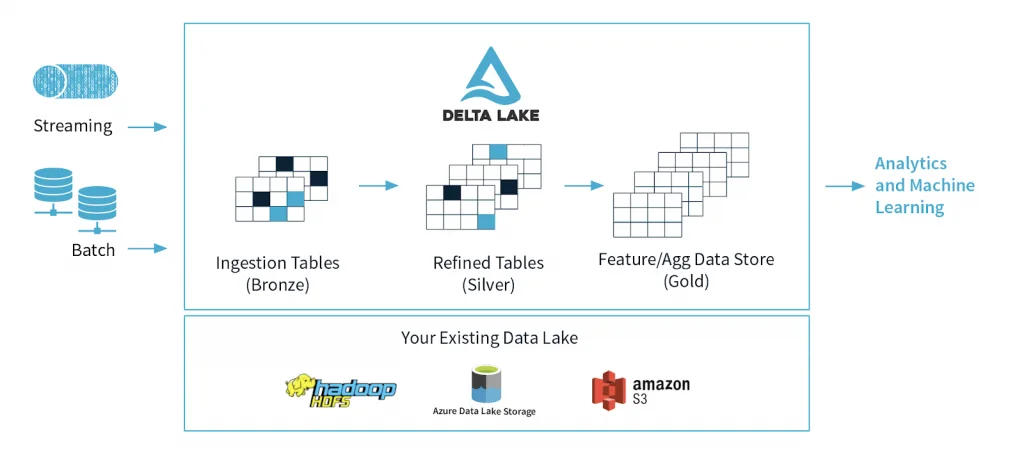
\includegraphics[width=\linewidth]{images/delta_lake_architecture.png}
\caption{Architecture multi-sauts de Delta Lake}\label{fig:delta-lake-architecture}
\end{figure}

\section{Principaux avantages et caractéristiques de Delta Lake}
\begin{itemize}
	\item[\textbullet] \textbf{Pistes d'audit et historique:}Dans Delta Lake, chaque écriture existe en tant que transaction et est enregistrée en série dans un journal des transactions. Par conséquent, toutes les modifications ou validations apportées au journal des transactions sont enregistrées, laissant une trace complète à utiliser dans les audits historiques, la gestion des versions ou à des fins de voyage dans le temps. Cette fonctionnalité de Delta Lake permet de garantir l'intégrité et la fiabilité des données pour les opérations de données d'entreprise.
	\item[\textbullet] \textbf{Voyager dans le temps et versionner les données:} Étant donné que chaque écriture crée une nouvelle version et stocke l'ancienne version dans le journal des transactions, les utilisateurs peuvent afficher/restaurer les anciennes versions de données en fournissant l'horodatage ou le numéro de version d'une table ou d'un répertoire existant à l'API de lecture Sparks\@. À l'aide du numéro de version fourni, Delta Lake construit ensuite un instantané complet de la version avec les informations fournies par le journal des transactions. Les retours en arrière et la gestion des versions jouent un rôle essentiel dans l'expérimentation de l'apprentissage automatique, où les scientifiques des données modifient de manière itérative les hyperparamètres pour former des modèles et peuvent revenir aux modifications si nécessaire.
	\item[\textbullet] \textbf{Unifie le traitement par lots et par flux:} Chaque table d'un Delta Lake est un puits de lot et de flux. Avec le streaming structuré Sparks, les organisations peuvent diffuser et traiter efficacement les données de streaming. De plus, grâce à la gestion efficace des métadonnées, à la facilité d'évolutivité et à la qualité ACID de chaque transaction, l'analyse en temps quasi réel devient possible sans utiliser une architecture de données à deux niveaux plus compliquée.
	\item[\textbullet] \textbf{Gestion efficace et évolutive des métadonnées:} Delta Lakes stocke les informations de métadonnées dans le journal des transactions et exploite la puissance de traitement distribuée de Spark pour traiter rapidement, lire et gérer efficacement de gros volumes de métadonnées de données, améliorant ainsi la gouvernance des données.
	\item[\textbullet] \textbf{transactions ACID:} Delta Lakes garantit que les utilisateurs voient toujours une vue de données cohérente dans une table ou un répertoire. Il garantit cela en capturant chaque modification effectuée dans un journal de transactions et en l'isolant au niveau d'isolation le plus fort, le niveau sérialisable. Au niveau sérialisable, chaque opération existante a et suit une séquence en série qui, lorsqu'elle est exécutée une par une, fournit le même résultat que celui indiqué dans le tableau.
	\item[\textbullet] \textbf{Opérations du langage de manipulation de données:} Delta Lakes prend en charge les opérations DML telles que les mises à jour, les suppressions et les fusions, qui jouent un rôle dans les opérations de données complexes telles que la capture de données de modification (CDC), les upserts en continu et la dimension à évolution lente (SCD). Des opérations comme CDC assurent la synchronisation des données dans tous les systèmes de données et minimisent le temps et les ressources consacrés aux opérations ELT. Par exemple, en utilisant le CDC, au lieu d'ETL toutes les données disponibles, seules les données récemment mises à jour depuis la dernière opération subissent une transformation.
	\item[\textbullet] \textbf{Schema Enforcement:} Delta Lakes effectue une validation automatique du schéma en vérifiant un ensemble de règles pour déterminer la compatibilité d'une écriture d'un DataFrame vers une table. L'une de ces règles est l'existence de toutes les colonnes DataFrame dans la table cible. Une occurrence d'une colonne supplémentaire ou manquante dans le DataFrame génère une erreur d'exception. Une autre règle est que le DataFrame et la table cible doivent contenir les mêmes types de colonnes, ce qui, sinon, déclenchera une exception. Delta Lake utilise également DDL (Data Definition Language) pour ajouter explicitement de nouvelles colonnes. Cette fonctionnalité de lac de données permet d'éviter l'ingestion de données incorrectes, garantissant ainsi une qualité élevée des données.
	\item[\textbullet] \textbf{Compatibilité avec l'API de Spark:} Delta Lake est basé sur Apache Spark et est entièrement compatible avec l'API Spark, qui permet de créer des pipelines de données volumineuses efficaces et fiables.
	\item[\textbullet] \textbf{Flexibilité et intégration:} Delta Lake est une couche de stockage open source et utilise le format Parquet pour stocker des fichiers de données, ce qui favorise le partage de données et facilite l'intégration avec d'autres technologies et stimule l'innovation.
\end{itemize}

\section{Trino}

Trino, anciennement connu sous le nom de Presto, est un moteur de requêtes SQL distribué et open-source. Il est conçu pour exécuter des requêtes interactives et analytiques à grande échelle sur des données hétérogènes et distribuées. Trino offre une grande polyvalence en permettant l'accès à différents types de sources de données, qu'il s'agisse de bases de données relationnelles, de systèmes de fichiers, de sources de données en temps réel ou de services de stockage cloud. Grâce à sa conception distribuée, Trino permet des performances élevées et une scalabilité horizontale, ce qui en fait un outil essentiel pour l'analyse des données dans notre solution.